
\documentclass [11pt]{report}

\usepackage{fancyhdr}
\usepackage [french]{babel}

\usepackage[utf8]{inputenc}
\usepackage[T1]{fontenc}
\usepackage{textcomp}
\usepackage{graphicx}
\usepackage[a4paper]{geometry}
\usepackage{titlepic}
\usepackage{boxedminipage}
\usepackage{listings}
\usepackage{minitoc}
\usepackage{footmisc}
\usepackage{color}
\usepackage{graphicx}
\usepackage{fancyvrb}

\usepackage{eso-pic}

\makeatletter
\newlength\@tempdim@x
\newlength\@tempdim@y
% structure des commandes :
%   #1 = deplacement selon x
%   #2 = deplacement selon y
%   #3 = texte à mettre
\newcommand\AtUpperLeftCorner[3]{%
\begingroup
\@tempdim@x=0cm
\@tempdim@y=\paperheight
\advance\@tempdim@x#1
\advance\@tempdim@y-#2
\put(\LenToUnit{\@tempdim@x},\LenToUnit{\@tempdim@y}){#3}%
\endgroup
}
\newcommand\AtUpperRightCorner[3]{%
\begingroup
\@tempdim@x=\paperwidth
\@tempdim@y=\paperheight
\advance\@tempdim@x-#1
\advance\@tempdim@y-#2
\put(\LenToUnit{\@tempdim@x},\LenToUnit{\@tempdim@y}){#3}%
\endgroup
}
\newcommand\AtLowerLeftCorner[3]{%
\begingroup
\@tempdim@x=0cm
\@tempdim@y=0cm
\advance\@tempdim@x#1
\advance\@tempdim@y#2
\put(\LenToUnit{\@tempdim@x},\LenToUnit{\@tempdim@y}){#3}%
\endgroup
}
\newcommand\AtLowerRightCorner[3]{%
\begingroup
\@tempdim@x=\paperwidth
\@tempdim@y=0cm
\advance\@tempdim@x-#1
\advance\@tempdim@y#2
\put(\LenToUnit{\@tempdim@x},\LenToUnit{\@tempdim@y}){#3}%
\endgroup
}
% ajout de texte ou d'images en haut à gauche, en haut à droite, etc.
\AddToShipoutPicture{%
\AtLowerRightCorner{3cm}{1cm}{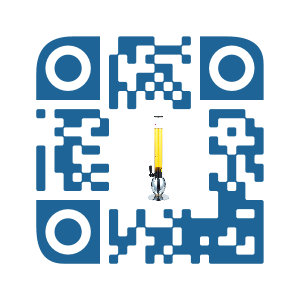
\includegraphics[scale=0.20]{images/LogoGroupe.png}}% image en bas à droite
}
\makeatother

\pagestyle{fancy}





\title{
	
\includegraphics[scale=0.43]{images/Logojeu.png}
	 \\\vspace{20mm}
	\textbf{\Huge \itshape Rapport de premi\`ere soutenance  }
	}




\author{ \\\vspace{2mm}
	Thibault Gdalia\\\vspace{2mm}
	Florent Youinou\\\vspace{2mm}
	Mathilde Laplaze\\\vspace{2mm}
	Vincent Baille \\\vspace{30mm}
	}


\date{17 janvier 2014}


\usepackage{listings,mdframed,xcolor}
\definecolor{codeBackground}{rgb}{0.95, 0.95, 0.95} %Couleur du rectangle%


\lstnewenvironment{mylisting}{
  \lstset{
  }
  \mdframed[backgroundcolor=codeBackground,shadow=false,shadowsize=2pt,shadowcolor=black!30]
}
{
  \endmdframed\ignorespaces
}


\begin{document}
\thispagestyle{fancy}
\renewcommand{\baselinestretch}{0.001}
\maketitle
\tableofcontents
\chapter*{Introduction} 
Dans le cadre de notre premi\`ere ann\'ee d'\'etude \`a EPITA, nous avons un projet informatique \`a r\'ealiser tout au long du deuxi\`eme semestre. Nous sommes au milieu de la p\'eriode pr\'evu pour la r\'ealisation de ce jeu. \\

Notre groupe de projet est toujours au complet, personne n'a quitt\'e l'\'ecole depuis la derni\`ere soutenance. Petit Rappel, notre \'equipe est compos\'ee de 4 membres: Mathilde "Mattou" Laplaze, Florent "T4ze" Youinou, Vincent "Vincae" Baille et Thibault "Skeat" Gdalia.Lors de ce deuxi\`eme rapport nous allons voir les diff\'erentes \'evolutions que nous avons apport\'e au jeu. Nous commencerons tout d'abord par rappeler ce que nous avions lors de la premi\`ere soutenance, l'\'etat du moteur physique, les diff\'erents mode de jeu et l'\'editeur de maps. Nous verrons par la suite les diff\'erents \'el\'ements que nous avons modif\'es, puis nous finirons sur les nouveaut\'es, c'est-\`a-dire ce qui n'exister pas avant.

\chapter{Ce que nous avions}
	\section{le diff\'erents mode de jeu}
		Lors de la soutenance pr\'ec\'edente, deux mode de jeu \'etait disponible: le mode story, et le mode infiny.
		\subsection{story}
			Dans ce mode de jeu, vous deviez parcourir une map jusqu'\'a la ligne d'arriv\'ee pour gagner mais si par malheur vous sortiez de l\'ecran par la gauche vous aviez perdu et deviez recommencer depuis le d\'ebut. Ce type de partie n'\'etait pas tr\'es int\'eressant car lorsque vous finissiez la map, vous aviez fini ce mode de jeu. Ce type de partie \'etait assez rapide \`a terminer, nous savions que pour rendre notre jeu plus attrayant il fallait que l'on modifie ce mode 
		\subsection{Infini}
			Ce mode de jeu est l\'eg\`rement diff\'erent, si la façon de jouer reste la m\^eme, le but du jeu n'est pas tout \'a fait pareil. Dans ce mode ci il faut tout d'abord avoir un compte que l'on a pr\'ealablement cr\'e'e sur notre site internet, il est tout fois possible de jouer sans compte mais cela perd un peu de son charme. Le but est d'aller le plus loin possible sur une map, les m\^etres que vous parcourez son comptabilis\'es. Lorsque vous avez touch\'e trop d'obstacles vous \^etes \'eject\'e de la map par la gauche, vous \^etes donc mort, le score est alors sauvegard\'e si vous n'avez jamais fait mieux, puis il est envoy\'e sur notre site web, o\'u vous trouvez un classement de tous les joueurs. vous pouvez ainsi d\'efier vos amis. \\
			\indent Sur ce mode de jeu, la map \'etait g\'en\'er\'ee al\'eatoirement, nous avions mis des probabilit\'es sur la possibilit\'e d'apparition pour que le jeu reste jouable. mais il n'y avait pas de r\'eelle coh\'erence dans l'apparition des blocs. Vous verrez que ce mode de jeu a reçu quelques modifications afin de le rendre encore plus agr\'eable \`a jouer\\
			\indent Nous avons apport\'e quelque modifications aux deux modes de jeu existant et nous en avons un nouveau, vous trouverez plus de d\'etails dans la suite du rapport dans les modifications, et dans les nouveaut\'es
	\section{Moteur physique}
		Le Moteur physique \'etait assez rudimentaire lors de la premi\`ere soutenance, lorsque l'on appuyait sur la barre espace l'oiseau effectuait un bond. Lorsqu'on ne touchait \`a rien, le personnage redescendait tranquillement en planant \`a l'aide de ses petites ailes. La façon dont nous avions cr\'e\'e les lois physique de notre jeu nous n'avions pas pr\'evu de changement possible en fonction de la map sur laquelle on se trouve, c'est principalement pour cette raison que nous avions d\'ecid\'e de refaire int\'egralement le moteur physique, nous entrerons dans les d\'etails de ces modifications plus tard dans ce rapport, dans la partie des modifications\\
		\indent Pour les collisions il y avait quelques probl\`emes dans certains cas, nous n'avions pas pris tous les cas en compte, par exemple lorsque l'oiseau touchait un bloc de face et qu'il avait un bloc au dessus de lui, il \'etait possible de traverser les blocs, ce probl\`eme permettait au joueur de tricher et d'\'eviter de mourir.
	\section{site internet}
		Notre site internet \'etait d\'ej\`a en ligne lors de la premi\`re soutenance, et il \'etait assez bien complet. vous pouvez trouver la description de notre projet, une pr\'esentation par membre de l'\'equipe, quelques photos du jeu, dans les t\'el\'echarchement vous pouvez r\'ecup\'erer le cahier des charges et le rapport de la soutenance 1, il y a aussi le classement des joueurs. Sur notre site vous pouvez aussi vous cr\'eer un compte.
	\section{graphisme}
	\section{son}
	\section{\'Editeur de maps}
		
	
\chapter{Les modifications}
\chapter{Les nouveaut\'ees}
\chapter{La suite}
\chapter*{Conclusion}




\end {document}